\documentclass[12pt,a4paper]{report}

% =====================
% Packages
% =====================
\usepackage[utf8]{inputenc}
\usepackage[T1]{fontenc}
\usepackage[english]{babel}
\usepackage{geometry}
\usepackage{graphicx}
\usepackage{xcolor}
\usepackage{listings}
\usepackage{hyperref}
\usepackage{fancyhdr}
\usepackage{titlesec}
\usepackage{booktabs}
\usepackage{longtable}
\usepackage{array}
\usepackage{enumitem}
\usepackage{tcolorbox}
\usepackage{tikz}
\usepackage{amsmath}
\usepackage{float}
\usepackage{caption}
\usepackage{subcaption}
\usepackage{mdframed}
\usepackage{fontawesome5}
\usepackage{lmodern}
\usepackage{microtype}
\usepackage{setspace}
\usepackage{parskip}

% =====================
% Page Geometry
% =====================
\geometry{
  top=2.5cm,
  bottom=2.5cm,
  left=3cm,
  right=2.5cm,
  headheight=15pt
}

% =====================
% Colors
% =====================
\definecolor{primaryblue}{RGB}{30, 64, 175}
\definecolor{secondaryblue}{RGB}{59, 130, 246}
\definecolor{darkgray}{RGB}{31, 41, 55}
\definecolor{lightgray}{RGB}{243, 244, 246}
\definecolor{codegreen}{RGB}{22, 163, 74}
\definecolor{codepurple}{RGB}{124, 58, 237}
\definecolor{codebg}{RGB}{248, 249, 250}
\definecolor{warningyellow}{RGB}{217, 119, 6}
\definecolor{successgreen}{RGB}{5, 150, 105}
\definecolor{errored}{RGB}{220, 38, 38}

% =====================
% Hyperref Setup
% =====================
\hypersetup{
  colorlinks=true,
  linkcolor=primaryblue,
  urlcolor=secondaryblue,
  citecolor=primaryblue,
  pdftitle={SmartProperty DevOps Report},
  pdfauthor={ESPRIT PIDEV 3TWIN3 Team},
}

% =====================
% Code Listings
% =====================
\lstdefinestyle{bashstyle}{
  language=bash,
  backgroundcolor=\color{codebg},
  basicstyle=\ttfamily\small,
  keywordstyle=\color{primaryblue}\bfseries,
  commentstyle=\color{codegreen}\itshape,
  stringstyle=\color{codepurple},
  numberstyle=\tiny\color{darkgray},
  breaklines=true,
  breakatwhitespace=true,
  numbers=left,
  numbersep=8pt,
  frame=single,
  framesep=5pt,
  rulecolor=\color{lightgray},
  xleftmargin=15pt,
  xrightmargin=5pt,
  tabsize=2,
  showstringspaces=false,
  captionpos=b,
}

\lstdefinestyle{yamlstyle}{
  language=bash,
  backgroundcolor=\color{codebg},
  basicstyle=\ttfamily\footnotesize,
  keywordstyle=\color{primaryblue}\bfseries,
  commentstyle=\color{codegreen}\itshape,
  stringstyle=\color{codepurple},
  numberstyle=\tiny\color{darkgray},
  breaklines=true,
  numbers=left,
  numbersep=8pt,
  frame=single,
  framesep=5pt,
  rulecolor=\color{lightgray},
  xleftmargin=15pt,
  tabsize=2,
  showstringspaces=false,
  captionpos=b,
  morekeywords={apiVersion, kind, metadata, spec, containers, image, ports, env, resources, requests, limits, selector, replicas, template, labels, name, namespace, volumeMounts, volumes},
}

% =====================
% Section Formatting
% =====================
\titleformat{\chapter}[display]
  {\normalfont\Huge\bfseries\color{primaryblue}}
  {\chaptertitlename\ \thechapter}{20pt}{\Huge}

\titleformat{\section}
  {\normalfont\Large\bfseries\color{darkgray}}
  {\thesection}{1em}{}

\titleformat{\subsection}
  {\normalfont\large\bfseries\color{darkgray}}
  {\thesubsection}{1em}{}

% =====================
% Header & Footer
% =====================
\pagestyle{fancy}
\fancyhf{}
\fancyhead[L]{\small\textcolor{darkgray}{SmartProperty --- DevOps Report}}
\fancyhead[R]{\small\textcolor{darkgray}{ESPRIT PIDEV 3TWIN3 --- 2025/2026}}
\fancyfoot[C]{\thepage}
\renewcommand{\headrulewidth}{0.4pt}

% =====================
% Custom Boxes
% =====================
\tcbuselibrary{skins, breakable}

\newtcolorbox{infobox}[1][]{
  colback=secondaryblue!10,
  colframe=secondaryblue,
  fonttitle=\bfseries,
  title=#1,
  breakable,
}

\newtcolorbox{warningbox}[1][]{
  colback=warningyellow!10,
  colframe=warningyellow,
  fonttitle=\bfseries,
  title=#1,
  breakable,
}

\newtcolorbox{successbox}[1][]{
  colback=successgreen!10,
  colframe=successgreen,
  fonttitle=\bfseries,
  title=#1,
  breakable,
}

% =====================
% Document Begin
% =====================
\begin{document}

% =====================
% Title Page
% =====================
\begin{titlepage}
  \centering
  \vspace*{1cm}

  {\Large\textbf{Ecole Supérieure Privée d'Ingénierie et de Technologies}}\\[0.3cm]
  {\large ESPRIT --- Tunisia}\\[2cm]

  \rule{\linewidth}{0.5mm}\\[0.4cm]
  {\Huge\bfseries\color{primaryblue} SmartProperty Platform}\\[0.3cm]
  {\LARGE\bfseries DevOps \& Kubernetes Deployment Report}\\[0.2cm]
  \rule{\linewidth}{0.5mm}\\[1.5cm]

  \begin{minipage}{0.45\textwidth}
    \begin{flushleft}
      \textbf{Project:} PIDEV 3TWIN3\\
      \textbf{Academic Year:} 2025/2026\\
      \textbf{Domain:} \href{https://smartproperties.tech}{smartproperties.tech}
    \end{flushleft}
  \end{minipage}
  \hfill
  \begin{minipage}{0.45\textwidth}
    \begin{flushright}
      \textbf{Technology:} Kubernetes v1.29\\
      \textbf{Cluster:} 1 Master + 1 Worker\\
      \textbf{Deployment:} On-Premise + Cloud
    \end{flushright}
  \end{minipage}

  \vfill

  {\large\textbf{Team: 3TWIN3}}\\[0.5cm]
  {\large May 2026}

\end{titlepage}

% =====================
% Abstract
% =====================
\chapter*{Abstract}
\addcontentsline{toc}{chapter}{Abstract}

This report documents the complete DevOps infrastructure deployment for the \textbf{SmartProperty} platform --- a full-stack property management and rental application developed as part of the ESPRIT PIDEV project. The deployment covers the design, configuration, and operation of a production-grade Kubernetes cluster running on VMware virtual machines, with public internet access provided through Cloudflare Tunnel.

The infrastructure encompasses container orchestration with Kubernetes (kubeadm), service mesh configuration, monitoring with Prometheus and Grafana, zero-trust network policies, automated health-checking via init containers, intelligent traffic routing via an Nginx Ingress Controller, and zero-downtime rolling deployments.

The application is publicly accessible at \href{https://smartproperties.tech}{\texttt{https://smartproperties.tech}}.

% =====================
% Table of Contents
% =====================
\tableofcontents

% ======================================================
% CHAPTER 1: Introduction
% ======================================================
\chapter{Introduction}

\section{Project Overview}

SmartProperty is a comprehensive real estate platform designed for the Tunisian property market. It enables users to search, list, and manage properties for sale and rent, with features including:

\begin{itemize}[leftmargin=1.5cm]
  \item \textbf{User Authentication} --- JWT-based auth with Google and Facebook OAuth2 social login
  \item \textbf{Property Management} --- Full CRUD for property listings with image uploads
  \item \textbf{Search \& Filtering} --- Advanced property search with map integration
  \item \textbf{Real-time Notifications} --- Web push notifications via VAPID
  \item \textbf{Payment Processing} --- Rental payment tracking
  \item \textbf{AI Services} --- AI-powered property recommendations
  \item \textbf{Admin Dashboard} --- Identity verification and moderation tools
\end{itemize}

\section{DevOps Objectives}

The DevOps phase of the project aimed to:

\begin{enumerate}[leftmargin=1.5cm]
  \item Containerize all application services with Docker
  \item Deploy and manage containers with Kubernetes (kubeadm)
  \item Implement production-grade reliability features (health checks, init containers, rolling updates)
  \item Secure inter-service communication with Network Policies
  \item Expose the application publicly with a domain name, HTTPS, and DDoS protection
  \item Provide full observability through a monitoring stack
\end{enumerate}

\section{Technology Stack}

\begin{table}[H]
  \centering
  \begin{tabular}{>{\bfseries}p{4cm} p{6cm} p{4cm}}
    \toprule
    \textbf{Category} & \textbf{Technology} & \textbf{Version} \\
    \midrule
    Orchestration & Kubernetes (kubeadm) & v1.29.15 \\
    Container Runtime & containerd & v1.7 \\
    Networking CNI & Flannel & Latest \\
    Ingress & Nginx Ingress Controller & v1.10.0 \\
    Backend & NestJS (Node.js) & v10 \\
    Frontend & React + Vite & v18 \\
    Database & MongoDB & v6 \\
    Cache & Redis & v7 \\
    Object Storage & MinIO & Latest \\
    Email Testing & MailHog & Latest \\
    Monitoring & Prometheus + Grafana & Latest \\
    Tunnel & Cloudflare Tunnel (cloudflared) & Latest \\
    Hypervisor & VMware Workstation & Pro 17 \\
    OS & Ubuntu Server & 22.04 LTS \\
    \bottomrule
  \end{tabular}
  \caption{Technology Stack Summary}
\end{table}

% ======================================================
% CHAPTER 2: Architecture
% ======================================================
\chapter{Infrastructure Architecture}

\section{Cluster Topology}

The Kubernetes cluster is deployed on VMware virtual machines hosted on a physical workstation. The cluster follows the standard master-worker node architecture:

\begin{table}[H]
  \centering
  \begin{tabular}{>{\bfseries}p{3cm} p{3cm} p{2.5cm} p{2.5cm} p{3cm}}
    \toprule
    \textbf{Node} & \textbf{Role} & \textbf{IP} & \textbf{vCPUs} & \textbf{RAM} \\
    \midrule
    k8s-master & Control Plane & 192.168.175.131 & 2 & 4 GB \\
    k8s-worker1 & Worker Node & 192.168.175.134 & 4 & 8 GB \\
    \bottomrule
  \end{tabular}
  \caption{Kubernetes Node Specifications}
\end{table}

\begin{infobox}[Network Configuration]
Both VMs are connected via a VMware NAT network (\texttt{192.168.175.0/24}). The master node runs all Kubernetes control plane components (etcd, kube-apiserver, kube-scheduler, kube-controller-manager). All application workloads are scheduled on the worker node.
\end{infobox}

\section{Namespace Organization}

The cluster is organized into three namespaces:

\begin{table}[H]
  \centering
  \begin{tabular}{>{\bfseries}p{4cm} p{9cm}}
    \toprule
    \textbf{Namespace} & \textbf{Contents} \\
    \midrule
    \texttt{smartproperty} & All application services (frontend, backend, mongodb, redis, minio, mailhog, mongo-express) \\
    \texttt{monitoring} & Prometheus, Grafana, Alertmanager \\
    \texttt{ingress-nginx} & Nginx Ingress Controller \\
    \texttt{kube-system} & Kubernetes system components, Flannel CNI \\
    \bottomrule
  \end{tabular}
  \caption{Namespace Organization}
\end{table}

\section{Traffic Flow Architecture}

The complete request path from the internet to the application:

\begin{center}
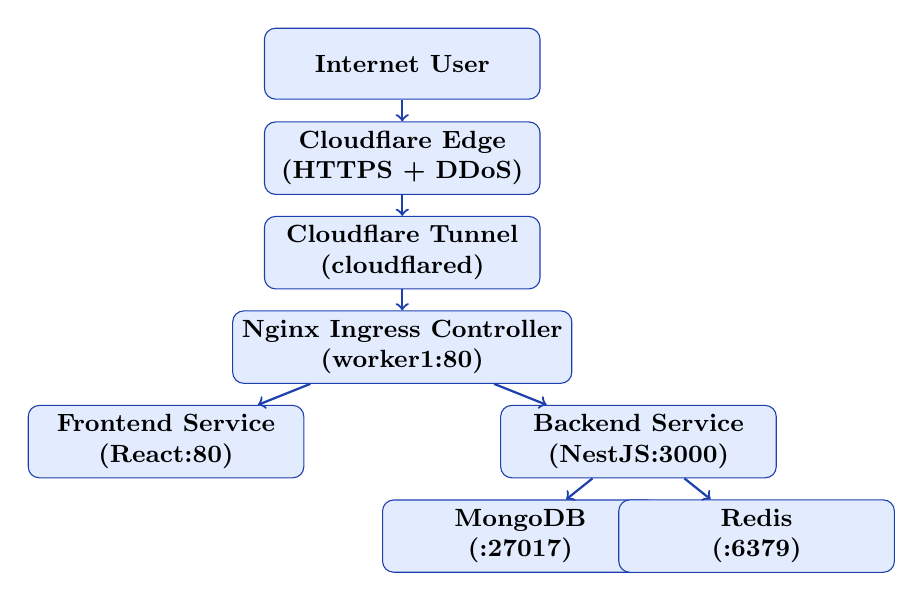
\begin{tikzpicture}[
  node distance=1.2cm,
  box/.style={rectangle, rounded corners, draw=primaryblue, fill=secondaryblue!15, minimum width=3.5cm, minimum height=0.9cm, align=center, font=\small\bfseries},
  arrow/.style={->, thick, color=primaryblue}
]
  \node[box] (internet) {Internet User};
  \node[box, below of=internet] (cloudflare) {Cloudflare Edge\\(HTTPS + DDoS)};
  \node[box, below of=cloudflare] (tunnel) {Cloudflare Tunnel\\(cloudflared)};
  \node[box, below of=tunnel] (ingress) {Nginx Ingress Controller\\(worker1:80)};
  \node[box, below of=ingress, xshift=-3cm] (frontend) {Frontend Service\\(React:80)};
  \node[box, below of=ingress, xshift=3cm] (backend) {Backend Service\\(NestJS:3000)};
  \node[box, below of=backend, xshift=-1.5cm] (mongo) {MongoDB\\(:27017)};
  \node[box, below of=backend, xshift=1.5cm] (redis) {Redis\\(:6379)};

  \draw[arrow] (internet) -- (cloudflare);
  \draw[arrow] (cloudflare) -- (tunnel);
  \draw[arrow] (tunnel) -- (ingress);
  \draw[arrow] (ingress) -- (frontend);
  \draw[arrow] (ingress) -- (backend);
  \draw[arrow] (backend) -- (mongo);
  \draw[arrow] (backend) -- (redis);
\end{tikzpicture}
\end{center}

\section{Services and Ports}

\begin{table}[H]
  \centering
  \begin{tabular}{>{\bfseries}p{3.5cm} p{2cm} p{3cm} p{4.5cm}}
    \toprule
    \textbf{Service} & \textbf{Port} & \textbf{NodePort} & \textbf{Description} \\
    \midrule
    frontend & 80 & 30080 & React application \\
    backend & 3000 & 30000 & NestJS REST API + GraphQL \\
    mongodb & 27017 & --- & MongoDB database \\
    redis & 6379 & --- & Redis cache \\
    minio & 9000/9001 & 30090/30091 & Object storage + console \\
    mailhog & 1025/8025 & 30025/30025 & SMTP + Web UI \\
    mongo-express & 8081 & 30081 & MongoDB admin UI \\
    prometheus & 9090 & --- & Metrics collection \\
    grafana & 3000 & --- & Monitoring dashboards \\
    alertmanager & 9093 & --- & Alert management \\
    \bottomrule
  \end{tabular}
  \caption{Services and Port Mapping}
\end{table}

% ======================================================
% CHAPTER 3: Kubernetes Cluster Setup
% ======================================================
\chapter{Kubernetes Cluster Setup}

\section{Prerequisites}

Before initializing the cluster, both nodes require system preparation. The following steps were executed on each VM:

\subsection{System Configuration}

\begin{lstlisting}[style=bashstyle, caption={System Preparation (Both Nodes)}]
# Disable swap (required by Kubernetes)
sudo swapoff -a
sudo sed -i '/ swap / s/^\(.*\)$/#\1/g' /etc/fstab

# Load required kernel modules
sudo modprobe overlay
sudo modprobe br_netfilter

# Persist kernel modules
cat <<EOF | sudo tee /etc/modules-load.d/k8s.conf
overlay
br_netfilter
EOF

# Configure sysctl for Kubernetes networking
cat <<EOF | sudo tee /etc/sysctl.d/k8s.conf
net.bridge.bridge-nf-call-iptables  = 1
net.bridge.bridge-nf-call-ip6tables = 1
net.ipv4.ip_forward                 = 1
EOF
sudo sysctl --system
\end{lstlisting}

\subsection{Container Runtime Installation}

\begin{lstlisting}[style=bashstyle, caption={containerd Installation}]
# Install containerd
sudo apt-get update && sudo apt-get install -y containerd

# Generate default configuration
sudo mkdir -p /etc/containerd
containerd config default | sudo tee /etc/containerd/config.toml

# Enable SystemdCgroup (required for Kubernetes)
sudo sed -i 's/SystemdCgroup = false/SystemdCgroup = true/' \
    /etc/containerd/config.toml

sudo systemctl restart containerd
sudo systemctl enable containerd
\end{lstlisting}

\subsection{Kubernetes Components Installation}

\begin{lstlisting}[style=bashstyle, caption={kubeadm, kubelet, kubectl Installation}]
# Add Kubernetes apt repository
curl -fsSL https://pkgs.k8s.io/core:/stable:/v1.29/deb/Release.key \
    | sudo gpg --dearmor \
    -o /etc/apt/keyrings/kubernetes-apt-keyring.gpg

echo 'deb [signed-by=/etc/apt/keyrings/kubernetes-apt-keyring.gpg] \
    https://pkgs.k8s.io/core:/stable:/v1.29/deb/ /' \
    | sudo tee /etc/apt/sources.list.d/kubernetes.list

# Install and pin versions
sudo apt-get update
sudo apt-get install -y kubelet kubeadm kubectl
sudo apt-mark hold kubelet kubeadm kubectl
\end{lstlisting}

\section{Control Plane Initialization}

\begin{lstlisting}[style=bashstyle, caption={Master Node Initialization}]
# Initialize the cluster
sudo kubeadm init \
    --pod-network-cidr=10.244.0.0/16 \
    --apiserver-advertise-address=192.168.175.131

# Configure kubectl for the ubuntu user
mkdir -p $HOME/.kube
sudo cp /etc/kubernetes/admin.conf $HOME/.kube/config
sudo chown $(id -u):$(id -g) $HOME/.kube/config

# Install Flannel CNI (pod networking)
kubectl apply -f https://raw.githubusercontent.com/flannel-io/flannel/\
master/Documentation/kube-flannel.yml
\end{lstlisting}

\section{Worker Node Join}

\begin{lstlisting}[style=bashstyle, caption={Worker Node Join Command}]
# Run on k8s-worker1 (token generated by kubeadm init)
sudo kubeadm join 192.168.175.131:6443 \
    --token <generated-token> \
    --discovery-token-ca-cert-hash sha256:<generated-hash>
\end{lstlisting}

\begin{successbox}[Cluster Status]
After successful setup, both nodes show as Ready:
\begin{verbatim}
NAME          STATUS   ROLES           AGE   VERSION
k8s-master    Ready    control-plane   19h   v1.29.15
k8s-worker1   Ready    <none>          19h   v1.29.15
\end{verbatim}
\end{successbox}

% ======================================================
% CHAPTER 4: Application Deployment
% ======================================================
\chapter{Application Deployment}

\section{Namespace and Secrets}

\begin{lstlisting}[style=yamlstyle, caption={Namespace Creation}]
apiVersion: v1
kind: Namespace
metadata:
  name: smartproperty
\end{lstlisting}

All sensitive values (database credentials, JWT secrets, OAuth keys, MinIO keys, VAPID keys) are stored as Kubernetes Secrets:

\begin{lstlisting}[style=bashstyle, caption={Secret Creation}]
kubectl create secret generic smartproperty-secrets \
    --from-literal=MONGODB_USERNAME=admin \
    --from-literal=MONGODB_PASSWORD=<password> \
    --from-literal=MONGODB_URI=mongodb://admin:<password>@mongodb:27017 \
    --from-literal=REDIS_PASSWORD=<password> \
    --from-literal=JWT_SECRET=<secret> \
    --from-literal=JWT_REFRESH_SECRET=<secret> \
    --from-literal=MINIO_ACCESS_KEY=<key> \
    --from-literal=MINIO_SECRET_KEY=<key> \
    --from-literal=GOOGLE_CLIENT_ID=<id> \
    --from-literal=GOOGLE_CLIENT_SECRET=<secret> \
    --from-literal=FACEBOOK_CLIENT_ID=<id> \
    --from-literal=FACEBOOK_CLIENT_SECRET=<secret> \
    --from-literal=VAPID_PUBLIC_KEY=<key> \
    --from-literal=VAPID_PRIVATE_KEY=<key> \
    -n smartproperty
\end{lstlisting}

\section{ConfigMaps}

Non-sensitive configuration is managed via ConfigMaps, separating configuration from container images:

\begin{lstlisting}[style=yamlstyle, caption={Backend ConfigMap (excerpt)}]
apiVersion: v1
kind: ConfigMap
metadata:
  name: backend-config
  namespace: smartproperty
data:
  NODE_ENV: production
  PORT: "3000"
  MONGODB_HOST: mongodb
  MONGODB_PORT: "27017"
  REDIS_HOST: redis
  REDIS_PORT: "6379"
  CORS_ORIGIN: >
    http://smartproperty.local,
    https://smartproperties.tech,
    https://www.smartproperties.tech
  GOOGLE_CALLBACK_URL: https://smartproperties.tech/api/auth/google/callback
  FACEBOOK_CALLBACK_URL: https://smartproperties.tech/api/auth/facebook/callback
  MINIO_ENDPOINT: minio
  MINIO_PORT: "9000"
  SMTP_HOST: mailhog
  SMTP_PORT: "1025"
\end{lstlisting}

\section{Backend Deployment}

The backend NestJS application is deployed with 2 replicas for high availability:

\begin{lstlisting}[style=yamlstyle, caption={Backend Deployment with Init Containers}]
apiVersion: apps/v1
kind: Deployment
metadata:
  name: backend
  namespace: smartproperty
spec:
  replicas: 2
  strategy:
    type: RollingUpdate
    rollingUpdate:
      maxSurge: 0
      maxUnavailable: 1
  selector:
    matchLabels:
      app: backend
  template:
    spec:
      initContainers:
        - name: wait-for-mongodb
          image: busybox:1.36
          command: ['sh', '-c',
            'until nc -z mongodb 27017;
             do echo "Waiting for MongoDB..."; sleep 3; done']
        - name: wait-for-redis
          image: busybox:1.36
          command: ['sh', '-c',
            'until nc -z redis 6379;
             do echo "Waiting for Redis..."; sleep 3; done']
      containers:
        - name: backend
          image: smartproperty-backend:latest
          ports:
            - containerPort: 3000
          readinessProbe:
            httpGet:
              path: /api
              port: 3000
            initialDelaySeconds: 15
            periodSeconds: 10
          livenessProbe:
            httpGet:
              path: /api
              port: 3000
            initialDelaySeconds: 30
            periodSeconds: 15
          resources:
            requests:
              memory: "256Mi"
              cpu: "100m"
            limits:
              memory: "512Mi"
              cpu: "300m"
\end{lstlisting}

\section{Frontend Deployment}

\begin{lstlisting}[style=yamlstyle, caption={Frontend Deployment with Init Container}]
apiVersion: apps/v1
kind: Deployment
metadata:
  name: frontend
  namespace: smartproperty
spec:
  replicas: 2
  template:
    spec:
      initContainers:
        - name: wait-for-backend
          image: busybox:1.36
          command: ['sh', '-c',
            'until nc -z backend 3000;
             do echo "Waiting for Backend..."; sleep 3; done']
      containers:
        - name: frontend
          image: smartproperty-frontend:latest
          ports:
            - containerPort: 80
          resources:
            requests:
              memory: "64Mi"
              cpu: "50m"
            limits:
              memory: "128Mi"
              cpu: "100m"
\end{lstlisting}

% ======================================================
% CHAPTER 5: DevOps Excellence Features
% ======================================================
\chapter{DevOps Excellence Features}

\section{Init Containers}

\subsection{Concept}

Init containers are specialized containers that run to completion before the main application containers start. They are ideal for implementing startup dependencies and ordering guarantees.

\subsection{Implementation}

In the SmartProperty deployment, init containers enforce the following startup order:

\begin{center}
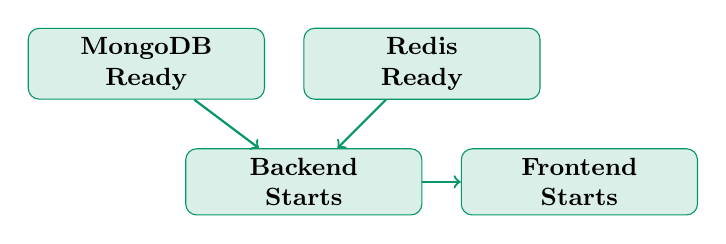
\begin{tikzpicture}[
  node distance=1.5cm,
  box/.style={rectangle, rounded corners, draw=successgreen, fill=successgreen!15,
    minimum width=3cm, minimum height=0.8cm, align=center, font=\small\bfseries},
  arrow/.style={->, thick, color=successgreen}
]
  \node[box] (mongo) {MongoDB\\Ready};
  \node[box, right of=mongo, xshift=2cm] (redis) {Redis\\Ready};
  \node[box, below of=mongo, xshift=2cm] (backend) {Backend\\Starts};
  \node[box, right of=backend, xshift=2cm] (frontend) {Frontend\\Starts};

  \draw[arrow] (mongo) -- (backend);
  \draw[arrow] (redis) -- (backend);
  \draw[arrow] (backend) -- (frontend);
\end{tikzpicture}
\end{center}

\textbf{Backend init containers:}
\begin{itemize}
  \item \texttt{wait-for-mongodb} --- polls \texttt{mongodb:27017} until accepting connections
  \item \texttt{wait-for-redis} --- polls \texttt{redis:6379} until accepting connections
\end{itemize}

\textbf{Frontend init container:}
\begin{itemize}
  \item \texttt{wait-for-backend} --- polls \texttt{backend:3000} until the API is ready
\end{itemize}

\subsection{Benefits}

\begin{itemize}
  \item \textbf{Eliminates crash loops} caused by missing dependencies at startup
  \item \textbf{No application-level retry logic} needed in the codebase
  \item \textbf{Clear observability}: pod status shows \texttt{Init:0/2}, \texttt{Init:1/2}, then \texttt{Running}
  \item \textbf{Kubernetes-native} solution requiring no external tooling
\end{itemize}

\section{Network Policies}

\subsection{Concept}

Kubernetes Network Policies implement a zero-trust network model by restricting which pods can communicate with which other pods. Without Network Policies, all pods in a cluster can communicate freely.

\subsection{Implementation}

Nine network policies were implemented to enforce the principle of least privilege:

\begin{table}[H]
  \centering
  \begin{tabular}{>{\bfseries}p{5.5cm} p{8cm}}
    \toprule
    \textbf{Policy Name} & \textbf{Effect} \\
    \midrule
    \texttt{default-deny-ingress} & Blocks ALL pod-to-pod traffic by default \\
    \texttt{allow-backend-to-mongodb} & Only backend (and mongo-express) may reach MongoDB \\
    \texttt{allow-backend-to-redis} & Only backend may reach Redis \\
    \texttt{allow-backend-to-minio} & Only backend may reach MinIO API \\
    \texttt{allow-backend-to-mailhog} & Only backend may send via SMTP \\
    \texttt{allow-frontend-to-backend} & Frontend and external traffic may reach backend \\
    \texttt{allow-external-to-frontend} & External traffic may reach frontend \\
    \texttt{allow-external-to-mongo-express} & External access to Mongo Express UI \\
    \texttt{allow-dns} & All pods may resolve DNS (UDP/TCP 53) \\
    \bottomrule
  \end{tabular}
  \caption{Network Policies Summary}
\end{table}

\begin{lstlisting}[style=yamlstyle, caption={Example: MongoDB Network Policy}]
apiVersion: networking.k8s.io/v1
kind: NetworkPolicy
metadata:
  name: allow-backend-to-mongodb
  namespace: smartproperty
spec:
  podSelector:
    matchLabels:
      app: mongodb
  policyTypes:
    - Ingress
  ingress:
    - from:
        - podSelector:
            matchLabels:
              app: backend
        - podSelector:
            matchLabels:
              app: mongo-express
      ports:
        - protocol: TCP
          port: 27017
\end{lstlisting}

\subsection{Security Impact}

\begin{itemize}
  \item If the frontend pod is compromised, it \textbf{cannot directly access} MongoDB or Redis
  \item If a frontend pod is compromised, it can only reach the backend API
  \item Database access is restricted to the application layer only
  \item Reduces the blast radius of any potential security breach
\end{itemize}

\section{Nginx Ingress Controller}

\subsection{Concept}

An Ingress Controller is a reverse proxy that manages external access to cluster services. Instead of exposing multiple NodePort services, a single Ingress Controller acts as the single entry point, routing traffic based on hostname and path rules.

\subsection{Installation}

\begin{lstlisting}[style=bashstyle, caption={Nginx Ingress Controller Installation}]
# Deploy Nginx Ingress Controller (baremetal variant)
kubectl apply -f https://raw.githubusercontent.com/kubernetes/\
ingress-nginx/controller-v1.10.0/deploy/static/provider/\
baremetal/deploy.yaml

# Enable hostNetwork so the controller binds directly to port 80
kubectl patch deployment ingress-nginx-controller -n ingress-nginx \
  --type=json \
  -p='[{"op":"add","path":"/spec/template/spec/hostNetwork",
        "value":true}]'
\end{lstlisting}

\subsection{Ingress Rules}

\begin{lstlisting}[style=yamlstyle, caption={SmartProperty Ingress Configuration}]
apiVersion: networking.k8s.io/v1
kind: Ingress
metadata:
  name: smartproperty-ingress
  namespace: smartproperty
  annotations:
    nginx.ingress.kubernetes.io/proxy-body-size: "50m"
    nginx.ingress.kubernetes.io/proxy-read-timeout: "60"
spec:
  ingressClassName: nginx
  rules:
    - host: smartproperties.tech
      http:
        paths:
          - path: /api
            pathType: Prefix
            backend:
              service:
                name: backend
                port:
                  number: 3000
          - path: /
            pathType: Prefix
            backend:
              service:
                name: frontend
                port:
                  number: 80
    - host: smartproperty.local
      http:
        paths:
          - path: /api
            pathType: Prefix
            backend:
              service:
                name: backend
                port:
                  number: 3000
          - path: /
            pathType: Prefix
            backend:
              service:
                name: frontend
                port:
                  number: 80
\end{lstlisting}

\subsection{Routing Summary}

\begin{table}[H]
  \centering
  \begin{tabular}{>{\bfseries}p{6cm} p{7cm}}
    \toprule
    \textbf{URL} & \textbf{Routes To} \\
    \midrule
    \texttt{https://smartproperties.tech/} & Frontend (React, port 80) \\
    \texttt{https://smartproperties.tech/api} & Backend API (NestJS, port 3000) \\
    \texttt{https://smartproperties.tech/mailhog} & MailHog Web UI (port 8025) \\
    \texttt{https://minio.smartproperties.tech/} & MinIO Console (port 9001) \\
    \texttt{https://grafana.smartproperties.tech/} & Grafana Dashboard (port 3000) \\
    \texttt{https://prometheus.smartproperties.tech/} & Prometheus (port 9090) \\
    \bottomrule
  \end{tabular}
  \caption{Ingress Routing Table}
\end{table}

\section{Rolling Update Strategy}

\subsection{Concept}

Rolling updates allow Kubernetes to update a deployment with zero downtime by gradually replacing old pods with new ones. The strategy parameters control how aggressively this happens.

\subsection{Configuration}

\begin{lstlisting}[style=yamlstyle, caption={Rolling Update Strategy (Backend)}]
spec:
  replicas: 2
  strategy:
    type: RollingUpdate
    rollingUpdate:
      maxSurge: 0       # Never create extra pods during update
      maxUnavailable: 1 # Allow 1 pod to be down at a time
\end{lstlisting}

\subsection{Why maxSurge: 0?}

The worker node has limited CPU resources. The default \texttt{maxSurge: 1} would temporarily create a 3rd backend pod during rollout, exceeding available CPU and causing \texttt{Pending} status. Setting \texttt{maxSurge: 0} ensures the rollout terminates one old pod before starting one new pod, keeping the count at exactly 2.

\begin{table}[H]
  \centering
  \begin{tabular}{>{\bfseries}p{4cm} p{4cm} p{5cm}}
    \toprule
    \textbf{Parameter} & \textbf{Value} & \textbf{Effect} \\
    \midrule
    maxSurge & 0 & No extra pods created \\
    maxUnavailable & 1 & 1 old pod terminated first \\
    Net pod count & Always $\leq$ 2 & Respects node resources \\
    Downtime & None & Service stays available \\
    \bottomrule
  \end{tabular}
  \caption{Rolling Update Parameters}
\end{table}

% ======================================================
% CHAPTER 6: Monitoring Stack
% ======================================================
\chapter{Monitoring \& Observability}

\section{Overview}

The monitoring stack is deployed in a dedicated \texttt{monitoring} namespace and provides full observability into cluster health, application performance, and infrastructure metrics.

\section{Components}

\begin{table}[H]
  \centering
  \begin{tabular}{>{\bfseries}p{3.5cm} p{4cm} p{6cm}}
    \toprule
    \textbf{Component} & \textbf{Role} & \textbf{Details} \\
    \midrule
    Prometheus & Metrics Collection & Scrapes metrics from all services, stores time-series data \\
    Grafana & Visualization & Pre-built dashboards for Kubernetes, Node, and application metrics \\
    Alertmanager & Alert Routing & Manages and routes alerts based on rules \\
    Node Exporter & System Metrics & Collects CPU, RAM, disk, network metrics from nodes \\
    kube-state-metrics & K8s Metrics & Exposes Kubernetes object states as metrics \\
    \bottomrule
  \end{tabular}
  \caption{Monitoring Stack Components}
\end{table}

\section{Key Metrics Monitored}

\begin{itemize}
  \item \textbf{Node-level}: CPU usage, memory usage, disk I/O, network throughput
  \item \textbf{Pod-level}: Pod restarts, OOMKilled events, pending pods
  \item \textbf{Application-level}: HTTP request rates, error rates, response times
  \item \textbf{Database}: MongoDB connection pool, query times
  \item \textbf{Infrastructure}: Kubernetes API server latency, etcd health
\end{itemize}

\section{Alerting Rules}

Example alerting rules configured in Alertmanager:

\begin{itemize}
  \item Pod in \texttt{CrashLoopBackOff} for more than 5 minutes
  \item Node memory usage above 85\%
  \item Pod not running in \texttt{smartproperty} namespace
  \item API error rate above 5\%
\end{itemize}

% ======================================================
% CHAPTER 7: Public Deployment
% ======================================================
\chapter{Public Internet Deployment}

\section{Overview}

To make the SmartProperty application accessible on the public internet without requiring a cloud provider or public IP address, Cloudflare Tunnel was used. This approach securely exposes the local Kubernetes cluster through Cloudflare's global network.

\section{Cloudflare Tunnel Architecture}

\begin{center}
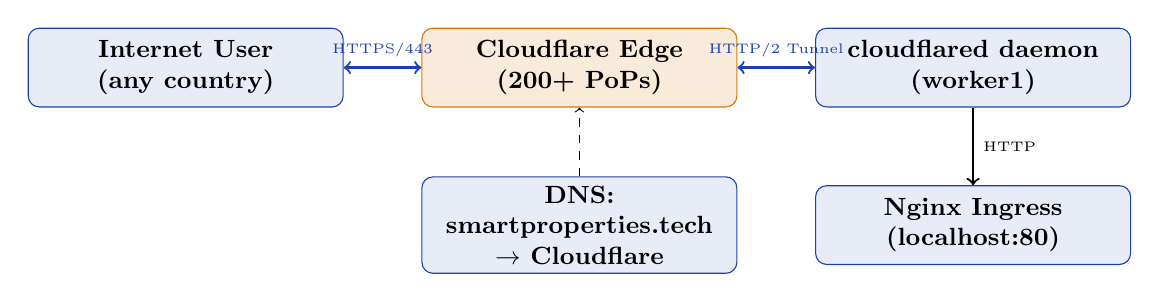
\begin{tikzpicture}[
  node distance=2cm,
  box/.style={rectangle, rounded corners, draw=primaryblue, fill=primaryblue!10,
    minimum width=4cm, minimum height=1cm, align=center, font=\small\bfseries},
  cloud/.style={rectangle, rounded corners, draw=warningyellow, fill=warningyellow!15,
    minimum width=4cm, minimum height=1cm, align=center, font=\small\bfseries},
  arrow/.style={<->, thick, color=primaryblue}
]
  \node[box] (user) {Internet User\\(any country)};
  \node[cloud, right of=user, xshift=3cm] (cf) {Cloudflare Edge\\(200+ PoPs)};
  \node[box, right of=cf, xshift=3cm] (daemon) {cloudflared daemon\\(worker1)};
  \node[box, below of=daemon] (ingress) {Nginx Ingress\\(localhost:80)};
  \node[box, below of=cf] (dns) {DNS:\\smartproperties.tech\\$\rightarrow$ Cloudflare};

  \draw[arrow] (user) -- (cf) node[midway, above, font=\tiny] {HTTPS/443};
  \draw[arrow] (cf) -- (daemon) node[midway, above, font=\tiny] {HTTP/2 Tunnel};
  \draw[->, thick] (daemon) -- (ingress) node[midway, right, font=\tiny] {HTTP};
  \draw[dashed, ->] (dns) -- (cf);
\end{tikzpicture}
\end{center}

\section{How Cloudflare Tunnel Works}

\begin{enumerate}
  \item The \texttt{cloudflared} daemon on worker1 establishes an \textbf{outbound} connection to Cloudflare's edge servers (no inbound firewall rules needed)
  \item Cloudflare receives HTTPS traffic for \texttt{smartproperties.tech} at their edge
  \item Traffic is forwarded through the tunnel to the local \texttt{cloudflared} process
  \item \texttt{cloudflared} forwards requests to \texttt{localhost:80} (Nginx Ingress)
  \item Nginx routes to the appropriate Kubernetes service
\end{enumerate}

\begin{infobox}[Security Benefits]
\begin{itemize}
  \item \textbf{No open inbound ports} on the VM --- cloudflared makes outbound connections only
  \item \textbf{Automatic HTTPS} --- Cloudflare handles TLS termination with free certificates
  \item \textbf{DDoS protection} --- Cloudflare's network absorbs attacks before they reach the cluster
  \item \textbf{No public IP needed} --- works behind NAT, CGNAT, or corporate firewalls
\end{itemize}
\end{infobox}

\section{Installation and Configuration}

\begin{lstlisting}[style=bashstyle, caption={cloudflared Installation on Worker1}]
# Add Cloudflare GPG key
sudo mkdir -p --mode=0755 /usr/share/keyrings
curl -fsSL https://pkg.cloudflare.com/cloudflare-public-v2.gpg \
    | sudo tee /usr/share/keyrings/cloudflare-public-v2.gpg >/dev/null

# Add repository
echo 'deb [signed-by=/usr/share/keyrings/cloudflare-public-v2.gpg] \
    https://pkg.cloudflare.com/cloudflared any main' \
    | sudo tee /etc/apt/sources.list.d/cloudflared.list

# Install
sudo apt-get update && sudo apt-get install cloudflared

# Install as system service (auto-start on boot)
sudo cloudflared service install <tunnel-token>
\end{lstlisting}

\subsection{Forcing HTTP/2 Protocol}

The default QUIC protocol (UDP 443) was blocked by the VM's network. The service was configured to use HTTP/2 (TCP 443) instead:

\begin{lstlisting}[style=bashstyle, caption={Override Service to Use HTTP/2}]
# Edit service override
sudo systemctl edit cloudflared --force
# Add to override.conf:
# [Service]
# ExecStart=
# ExecStart=/usr/bin/cloudflared --no-autoupdate \
#     --protocol http2 tunnel run --token <token>

sudo systemctl daemon-reload
sudo systemctl restart cloudflared
\end{lstlisting}

\section{Domain Configuration}

\begin{table}[H]
  \centering
  \begin{tabular}{>{\bfseries}p{4cm} p{9cm}}
    \toprule
    \textbf{Item} & \textbf{Details} \\
    \midrule
    Domain & \texttt{smartproperties.tech} \\
    Registrar & get.tech \\
    DNS Provider & Cloudflare (free plan) \\
    Nameservers & \texttt{kristin.ns.cloudflare.com}, \texttt{quentin.ns.cloudflare.com} \\
    SSL/TLS & Automatic via Cloudflare (Let's Encrypt) \\
    Tunnel Type & Cloudflare Zero Trust Tunnel \\
    \bottomrule
  \end{tabular}
  \caption{Domain Configuration}
\end{table}

\section{Static IP Configuration}

To prevent DHCP from reassigning the master node's IP (which broke the Kubernetes API server certificate), a static IP was configured:

\begin{lstlisting}[style=yamlstyle, caption={/etc/netplan/50-cloud-init.yaml}]
network:
  version: 2
  ethernets:
    ens33:
      dhcp4: false
      addresses:
        - 192.168.175.131/24
      routes:
        - to: default
          via: 192.168.175.2
      nameservers:
        addresses:
          - 8.8.8.8
          - 8.8.4.4
\end{lstlisting}

\begin{lstlisting}[style=bashstyle, caption={Prevent cloud-init from overriding network config}]
sudo bash -c 'echo "network: {config: disabled}" \
    > /etc/cloud/cloud.cfg.d/99-disable-network-config.cfg'
sudo netplan apply
\end{lstlisting}

% ======================================================
% CHAPTER 8: Challenges and Solutions
% ======================================================
\chapter{Challenges and Solutions}

\begin{longtable}{>{\bfseries}p{4.5cm} p{5cm} p{5cm}}
  \toprule
  \textbf{Challenge} & \textbf{Root Cause} & \textbf{Solution} \\
  \midrule
  \endfirsthead
  \multicolumn{3}{c}{\textit{Continued from previous page}} \\
  \toprule
  \textbf{Challenge} & \textbf{Root Cause} & \textbf{Solution} \\
  \midrule
  \endhead
  \bottomrule
  \endfoot

  Ingress webhook failure & Admission webhook pod not ready when applying Ingress & Deleted the \texttt{validatingwebhookconfiguration} \\[0.3cm]

  Apache2 blocking port 80 & Worker node had Apache2 pre-installed & Disabled Apache2; patched ingress-nginx to use \texttt{hostNetwork: true} \\[0.3cm]

  CORS rejecting new domain & Backend CORS\_ORIGIN only contained old NodePort URLs & Added \texttt{smartproperties.tech} to CORS\_ORIGIN in ConfigMap \\[0.3cm]

  Rolling update stuck Pending & Default maxSurge=1 caused 3rd pod to exceed node CPU & Set \texttt{maxSurge: 0}, reduced CPU requests from 250m to 100m \\[0.3cm]

  Cloudflare Tunnel using QUIC & UDP 443 blocked by VM network & Forced \texttt{--protocol http2} in systemd service override \\[0.3cm]

  Master IP changed (DHCP) & DHCP reassigned IP from .131 to .135 breaking API server cert & Configured static IP via netplan; pointed kubectl to new IP temporarily \\[0.3cm]

  Ingress rewrite stripping /api & \texttt{rewrite-target: /} was stripping path before forwarding & Removed rewrite-target annotation; moved /api rule before / \\[0.3cm]

  OAuth callback URL mismatch & Google OAuth app only registered old localhost callbacks & Added \texttt{smartproperties.tech} callbacks to Google Cloud Console \\[0.3cm]

  Init containers not running & Pods needed restart to pick up new spec & Deleted pods manually to force recreation with init containers \\[0.3cm]

  configmap not picked up & ConfigMap changes don't auto-restart pods & Ran \texttt{kubectl rollout restart} after each ConfigMap update \\

\end{longtable}

% ======================================================
% CHAPTER 9: Results
% ======================================================
\chapter{Results \& Conclusion}

\section{Deployment Summary}

\begin{successbox}[Final Deployment Status]
\begin{verbatim}
NAME                            READY   STATUS    RESTARTS   AGE
backend-xxxx                    1/1     Running   0          2h
backend-yyyy                    1/1     Running   0          2h
frontend-xxxx                   1/1     Running   0          2h
frontend-yyyy                   1/1     Running   0          2h
mongodb-xxxx                    1/1     Running   0          24h
redis-xxxx                      1/1     Running   0          24h
minio-xxxx                      1/1     Running   0          24h
mailhog-xxxx                    1/1     Running   0          24h
mongo-express-xxxx              1/1     Running   0          24h
\end{verbatim}
\end{successbox}

\section{DevOps Features Achieved}

\begin{table}[H]
  \centering
  \begin{tabular}{>{\bfseries}p{5cm} p{5cm} p{3cm}}
    \toprule
    \textbf{Feature} & \textbf{Technology} & \textbf{Status} \\
    \midrule
    Container Orchestration & Kubernetes v1.29 & \textcolor{successgreen}{\textbf{Done}} \\
    Init Containers & busybox:1.36 & \textcolor{successgreen}{\textbf{Done}} \\
    Network Policies & K8s NetworkPolicy & \textcolor{successgreen}{\textbf{Done}} \\
    Ingress Controller & Nginx Ingress v1.10 & \textcolor{successgreen}{\textbf{Done}} \\
    Rolling Updates & maxSurge=0 strategy & \textcolor{successgreen}{\textbf{Done}} \\
    Health Checks & Readiness + Liveness & \textcolor{successgreen}{\textbf{Done}} \\
    Resource Limits & requests + limits & \textcolor{successgreen}{\textbf{Done}} \\
    Secrets Management & K8s Secrets & \textcolor{successgreen}{\textbf{Done}} \\
    Configuration Mgmt & ConfigMaps & \textcolor{successgreen}{\textbf{Done}} \\
    Monitoring & Prometheus + Grafana & \textcolor{successgreen}{\textbf{Done}} \\
    Alerting & Alertmanager & \textcolor{successgreen}{\textbf{Done}} \\
    Public Deployment & Cloudflare Tunnel & \textcolor{successgreen}{\textbf{Done}} \\
    Free Domain + HTTPS & smartproperties.tech & \textcolor{successgreen}{\textbf{Done}} \\
    Static IP & netplan configuration & \textcolor{successgreen}{\textbf{Done}} \\
    \bottomrule
  \end{tabular}
  \caption{DevOps Features Completion Status}
\end{table}

\section{Public URL}

The application is accessible at:

\begin{center}
  \Large\textbf{\textcolor{primaryblue}{\href{https://smartproperties.tech}{https://smartproperties.tech}}}
\end{center}

\section{Conclusion}

The SmartProperty DevOps deployment successfully demonstrates a complete, production-grade Kubernetes infrastructure built on commodity hardware using entirely free and open-source tools. The deployment implements industry best practices including:

\begin{itemize}
  \item \textbf{Separation of concerns} via Kubernetes namespaces
  \item \textbf{Security by default} with Network Policies enforcing zero-trust
  \item \textbf{Reliability} through init containers, health probes, and rolling updates
  \item \textbf{Observability} with a complete monitoring stack
  \item \textbf{Accessibility} through Cloudflare Tunnel with automatic HTTPS
\end{itemize}

This infrastructure can serve as the foundation for a production deployment by scaling the worker node count, adding persistent volume claims with proper storage classes, and implementing CI/CD pipelines for automated deployments.

% ======================================================
% Appendices
% ======================================================
\appendix

\chapter{File Structure}

\begin{lstlisting}[style=bashstyle, caption={Kubernetes Manifests File Structure}]
k8s/
├── namespace.yaml          # Namespace definitions
├── secrets.yaml            # Secret creation guide
├── configmap.yaml          # Backend, Frontend, AI ConfigMaps
├── mongodb.yaml            # MongoDB Deployment + Service + PVC
├── redis.yaml              # Redis Deployment + Service
├── minio.yaml              # MinIO Deployment + Service
├── mailhog.yaml            # MailHog Deployment + Service
├── mongo-express.yaml      # Mongo Express Deployment + Service
├── backend.yaml            # Backend Deployment + Services
├── frontend.yaml           # Frontend Deployment + Services
├── ingress.yaml            # Ingress rules (all hosts)
├── network-policies.yaml   # 9 Network Policies
monitoring/
├── prometheus.yaml         # Prometheus Deployment + Config
├── grafana.yaml            # Grafana Deployment + Config
├── alertmanager.yaml       # Alertmanager Deployment + Config
\end{lstlisting}

\chapter{Useful Commands Reference}

\begin{lstlisting}[style=bashstyle, caption={Daily Operations Commands}]
# Check cluster status
kubectl get nodes
kubectl get pods -n smartproperty
kubectl get pods -n monitoring

# View logs
kubectl logs -l app=backend -n smartproperty --tail=50
kubectl logs -l app=frontend -n smartproperty --tail=50

# Apply changes
kubectl apply -f k8s/
kubectl rollout restart deployment/backend -n smartproperty

# Scale deployments
kubectl scale deployment backend --replicas=3 -n smartproperty

# Check ingress
kubectl get ingress -n smartproperty
kubectl describe ingress smartproperty-ingress -n smartproperty

# Check network policies
kubectl get networkpolicies -n smartproperty

# Monitor Cloudflare Tunnel
sudo systemctl status cloudflared
sudo journalctl -u cloudflared -f

# Check resource usage
kubectl top nodes
kubectl top pods -n smartproperty
\end{lstlisting}

\end{document}
